\chapter{Obogatitev besed}
\label{ch:obogatitev-besed}

Sedaj o modelu vemo že veliko, ampak kaj ne bi bilo super pogledati, za katere pravljice se je model zmotil in za katere je imel prav? Gradnik \widget{Confusion Matrix} omogoča prav to!

\begin{figure}[h]
    \centering
    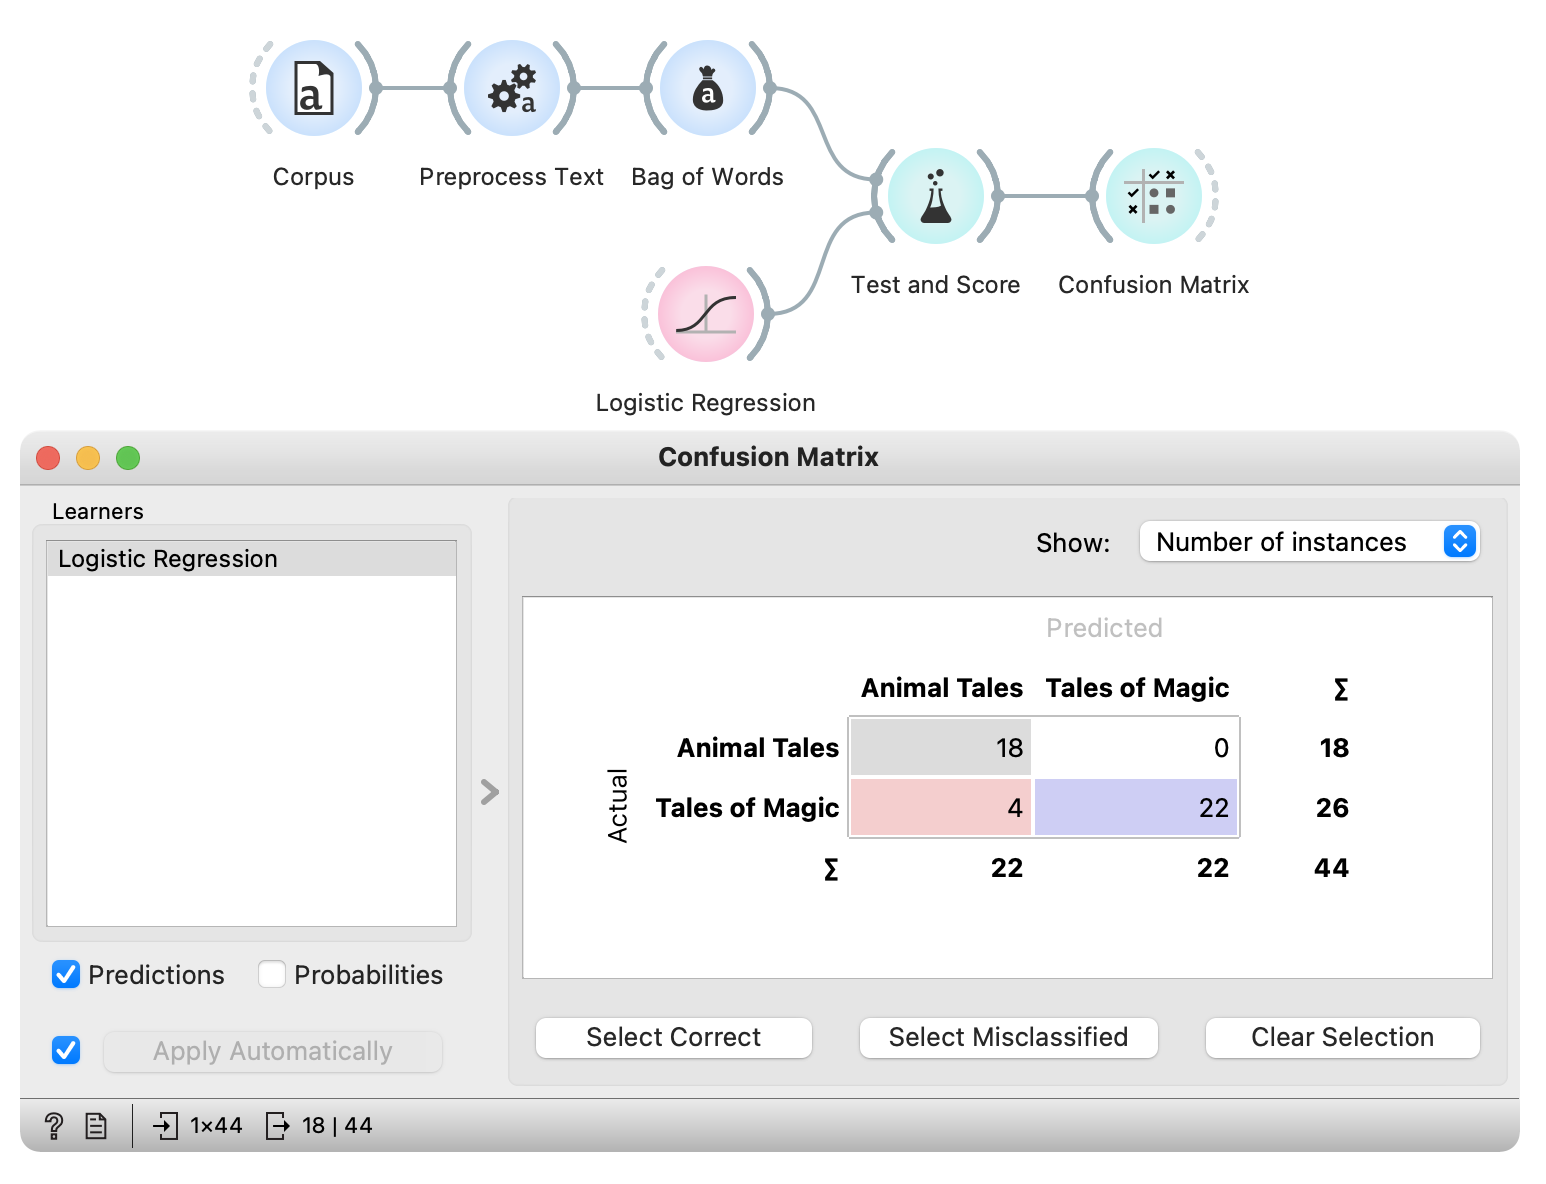
\includegraphics[width=\linewidth]{confusion-matrix.png}%
    \caption{Posamezne napačno klasificirane pravljice pogledamo s klikom na polje v tabeli.

    Vse napačno klasificirane dokumente lahko izberemo z gumbom ‘Select Misclassified’. To bo na izhod poslalo vse napačno klasificirane pravljice, ki jih nato pogledamo v gradniku Corpus Viewer.}
    \label{fig:009-confusion-matrix}
  \end{figure}
  
Tabela vsebuje pravilno napovedane dokumente v diagonali (modra) in nepravilno napovedane dokumente izven diagonale (rdeča). Vidimo, da so bile 4 magične pravljice napovedane kot živalske, medtem ko model ni nobene živalske napovedal kot magične.

Ampak zakaj? Kaj zaznamuje posamezno skupino pravljic, da jih lahko model pravilno razvrsti v pravi razred?

Da preverimo pravilno klasificirane dokumente, lahko uporabimo \widget{Corpus Viewer}. Ali pa še bolje, pogledamo, katere besede so značilne za katero podmnožico!

Obogatitev besed primerja podmnožico dokumentov s celotnim korpusom in odkrije besede, ki statistično signifikantno zaznamujejo izbrano podmnožico. 

\newpage

\begin{figure*}[h]
    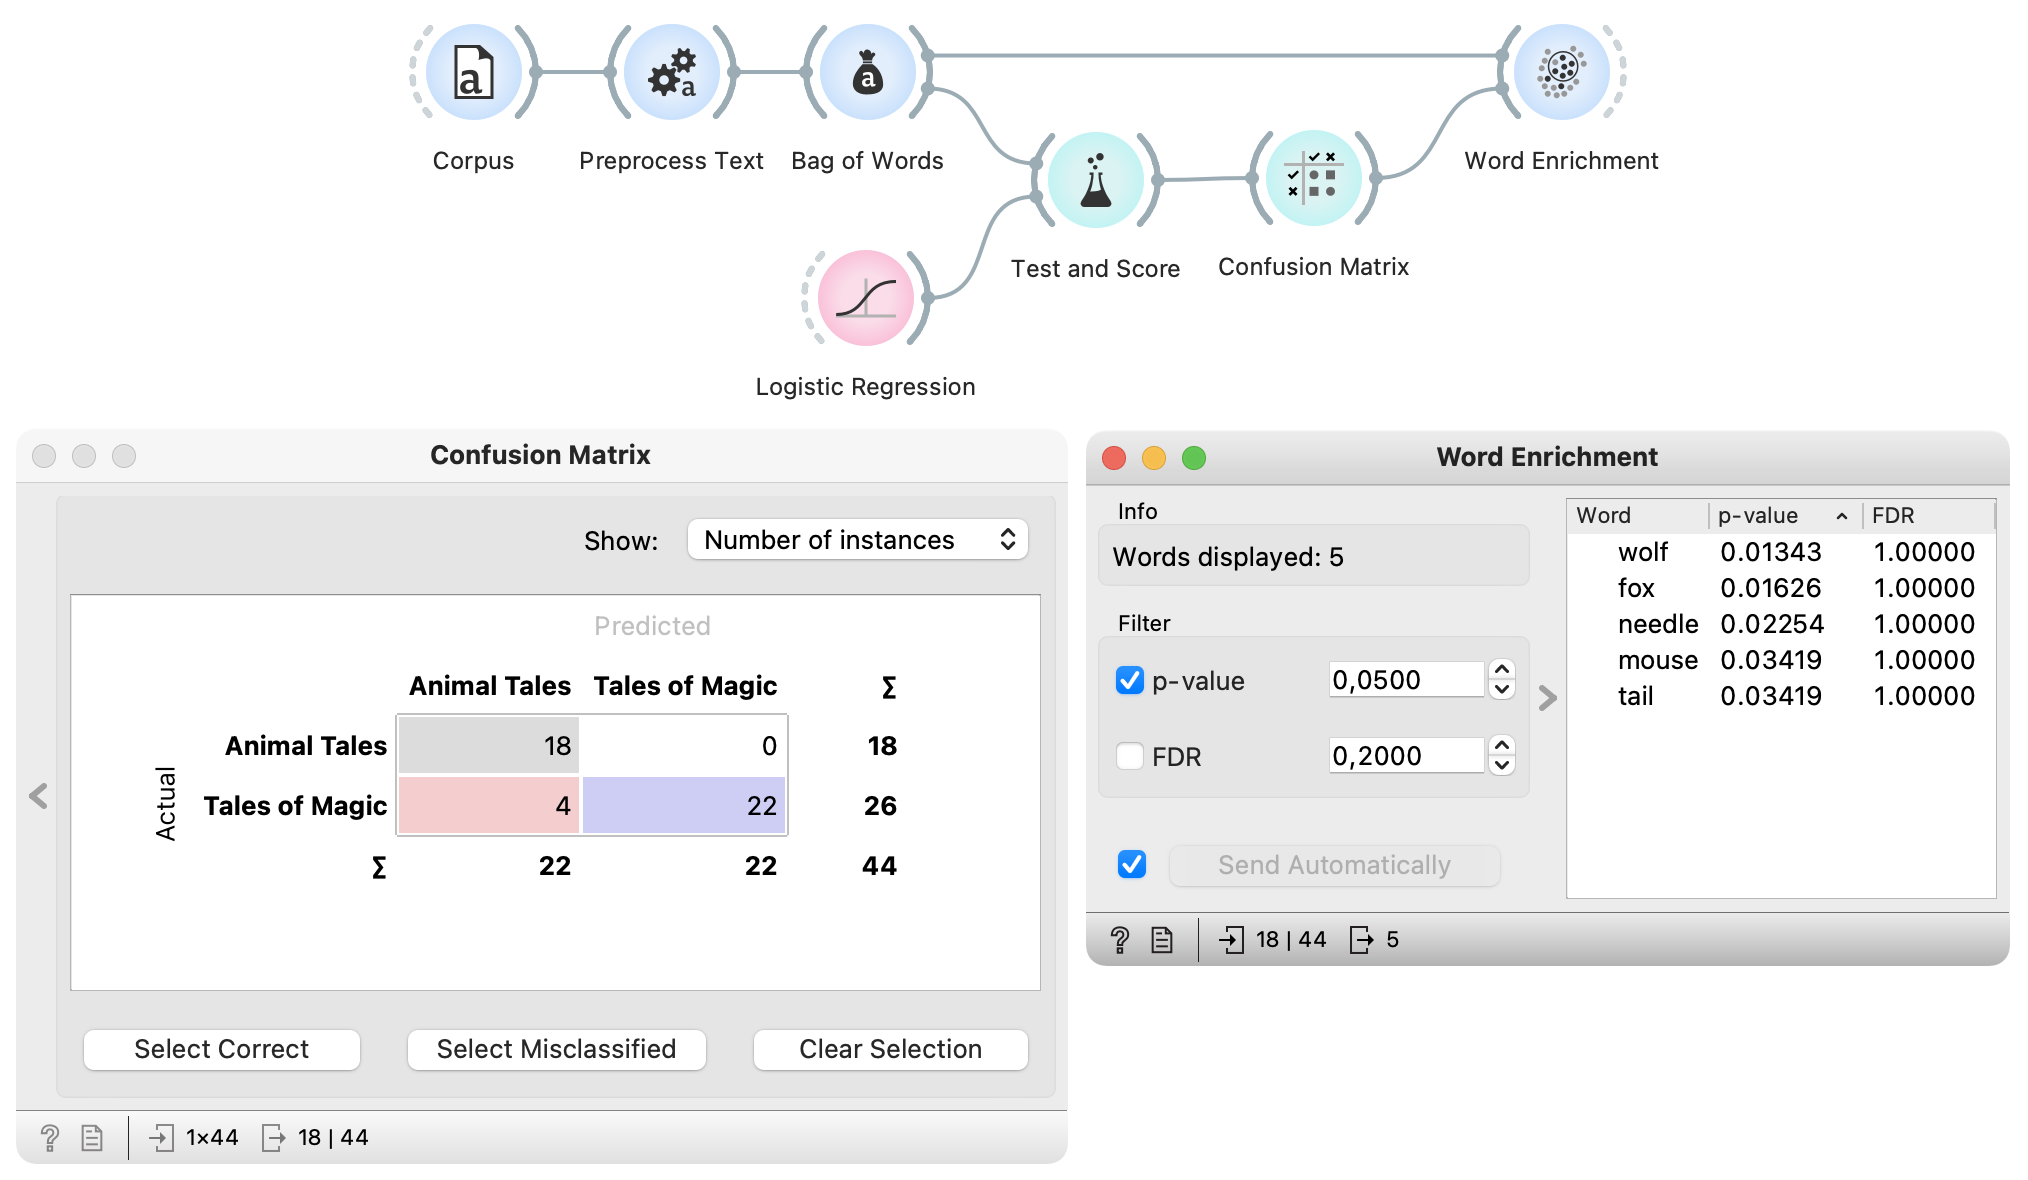
\includegraphics[width=\linewidth]{word-enrichment.png}%
    \caption{Word Enrichment deluje na kakršni koli podmnožici. V gradniku Corpus Viewer poiščite vse dokumente, ki vsebujejo besedo ‘queen’. Sedaj pošljite izbor v Word Enrichment. Ne pozabite povezati celotnega korpusa iz gradnika Bag of Words - Word Enrichment potrebuje celoten korpus za primerjavo.}
    \label{fig:009-word-enrichment}
\end{figure*}

Besedi ‘wolf’ in ‘fox’ najbolj zaznamujta pravilno napovedane živalske pravljice. Seznam je nekoliko daljši za pravilno napovedane magične pravljice -- ‘king’, ‘beautiful’, ‘man’, itd. Rezultati so zelo podobni tistim iz nomograma. Pravzaprav je to samo drugačen način, kako raziščemo model!

Torej ko boste naslednjič videli lisico v besedilu, ste lahko precej prepričani, da gre za živalsko pravljico! :)
  